\documentclass{article} % For LaTeX2e
% We will use NIPS submission format
\usepackage{nips13submit_e,times}
% for hyperlinks
\usepackage{hyperref}
\usepackage{url}
% For figures
\usepackage{graphicx} 
\usepackage{subfigure} 
% math packages
\usepackage{amsmath}
\usepackage{amsfonts}
\usepackage{amsopn}
\usepackage{ifthen}
\usepackage{natbib}

\title{Project-I by Group MUMBAI}

\author{
Audrey Loeffel\\
EPFL \\
\texttt{audrey.loeffel@epfl.ch} \\
\And 
Meryem M'hamdi\\
EPFL \\
\texttt{meryem.mhamdi@epfl.ch} \\
}

% The \author macro works with any number of authors. There are two commands
% used to separate the names and addresses of multiple authors: \And and \AND.
%
% Using \And between authors leaves it to \LaTeX{} to determine where to break
% the lines. Using \AND forces a linebreak at that point. So, if \LaTeX{}
% puts 3 of 4 authors names on the first line, and the last on the second
% line, try using \AND instead of \And before the third author name.

\nipsfinalcopy 

\begin{document}

\maketitle

\begin{abstract} 
In this report, we summarize our findings for project I applied on two Mumbai data sets. We started by analyzing the characteristics of our data, cleaning it using normalization and dummy encoding and investigating the nature of correlations between input and output data. In our regression data, we observed that three clusters exist; therefore, we needed to use logistic regression to classify our data and choose ridge regression for the best model. We also opted for logistic regression for classification data set and used cross validation with different values of alpha to minimize 0-1 loss error. 

\end{abstract}

\section{Data Description}
Our regression data contains input variables $\mathbf{X\_train}$  and output variables $\mathbf{y\_train}$ for training. We have $N=2800$ data examples of dimensionality $D=73$ and type double. 
Our data consists of 61 real valued variables and 12 categorical variables. Out of these 12 variables, 4 are binary, 5 have three categories and 3 have four categories.

Test-data is provided as $\mathbf{X\_test}$ but its corresponding output is not given. Only $N=1200$ testing data examples are provided.

Our classification data consists of input $\mathbf{X\_train}$ of size $N=1500$ and dimensionality  $D=28$ and its corresponding output $\mathbf{y\_train}$ provided for training purposes. Our classification input consists of 23 real valued variables and 5 categorical variables. Out of these 5 variables, two have 2 categories, one has 3 categories and two have 5 categories. The values of $\mathbf{y\_train}$ are either -1 or 1 making our data fall into 2 categories. 

\section{Exploratory data analysis, visualization and cleaning}

To learn about the characteristics of our input data, we examined closely how its variables are distributed. Figure \ref{fig:scatterPlotReg} shows the scatter plot of our data before normalization. \ref{fig:boxPlotB} shows that the data is not centred around 0, which means we need to normalize it. Figure \ref{fig:boxPlotA} displays our data distribution after transforming it to have zero mean and unit variance. 

\begin{figure}[!h]
\center
\subfigure[Scatter Plot of Regression Output $\mathbf{y\_train}$ Before Normalization]{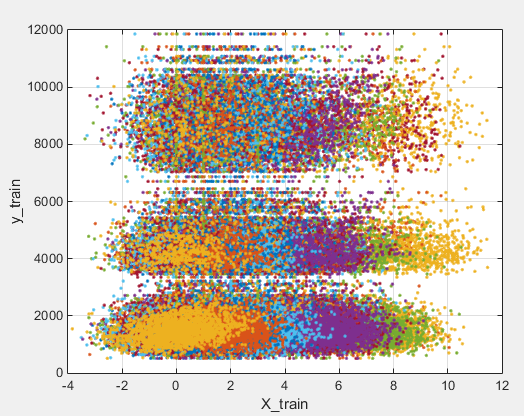
\includegraphics[width=2.5in]{figures/ScatterPlotReg.PNG} \label{fig:scatterPlotReg}}
\subfigure[Boxplot of real-valued $\mathbf{X\_train}$ before normalization.]{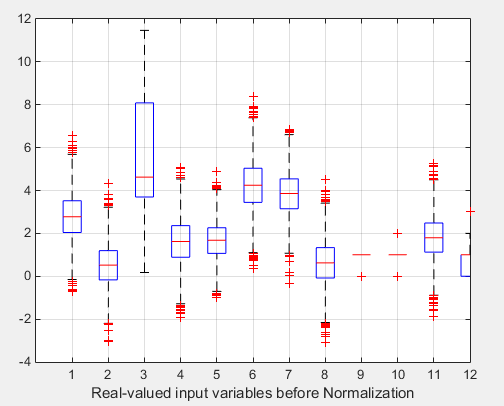
\includegraphics[width=2.5in]{figures/BoxPlotB.PNG} \label{fig:boxPlotB}}
\subfigure[Scatter Plot of Regression Output $\mathbf{y\_train}$ After Normalization]{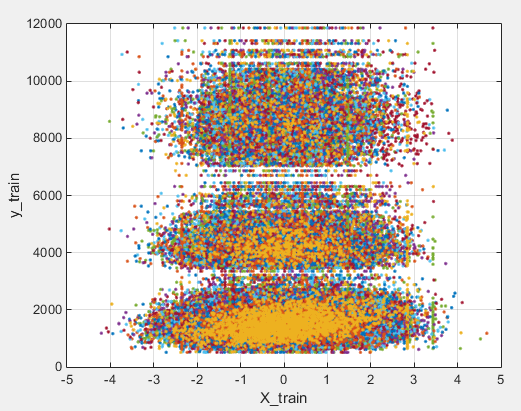
\includegraphics[width=2.5in]{figures/ScatterPlotRegAfterNorm.PNG} \label{fig:scatterPlotRegAfterNorm}}
\subfigure[Boxplot of data after normalization]{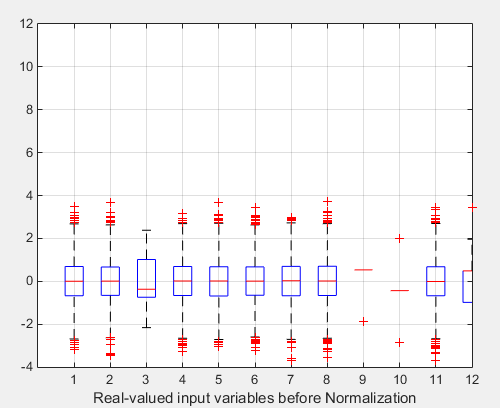
\includegraphics[width=2.7in]{figures/BoxPlotA.PNG} \label{fig:boxPlotA}}
\subfigure[Histogram of regression output data $\mathbf{y\_train}$]{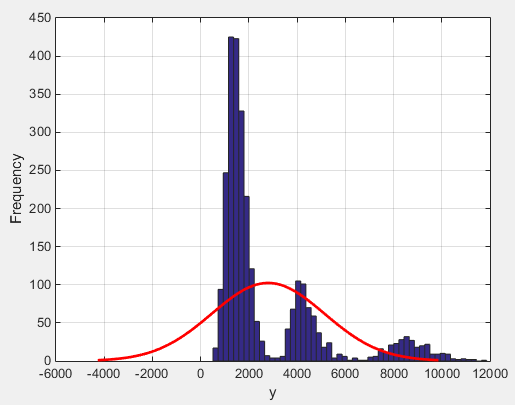
\includegraphics[width=2.5in]{figures/histReg.PNG} \label{fig:histReg}}
\hfill
\caption{Exploratory Data Analysis and Normalization}
\end{figure}


From the scatter plot of y with respect to X shown in figure \ref{fig:scatterPlotRegAfterNorm}, we observed that our data contains three distinct clouds. The histogram of the output y in figure \ref{fig:histReg} confirms the presence of three clusters. The distribution is clearly not Gaussian overall but the distributions of the three clusters are definitely Gaussian. This implies that our input data is not fully correlated with our output therefore instead of finding one model to fit the whole training set, we need to find three models to fit each cluster separately. For any new testing point, we choose the best model to be used by determining the cluster to which the point belongs to using logistic regression.  

We computed the correlation of each feature's outputs with the input for each cluster as shown in figure \ref{fig:corr}.  We observed that some features seem more correlated and can be interesting to use for feature transformation. Figure \ref{fig:ft46} shows a plot of a feature with a higher correlation between cluster 2\footnote{\samepage We named the clusters as cluster 1 has the lower outputs, cluster 3 has the higher outputs ans cluster 2is between 1 and 3.} and the outputs $\mathbf{y\_train}$.

\begin{figure}[!h]
\center
\subfigure[Bar chart of correlation between each cluster of each feature and $\mathbf{y\_train}$]{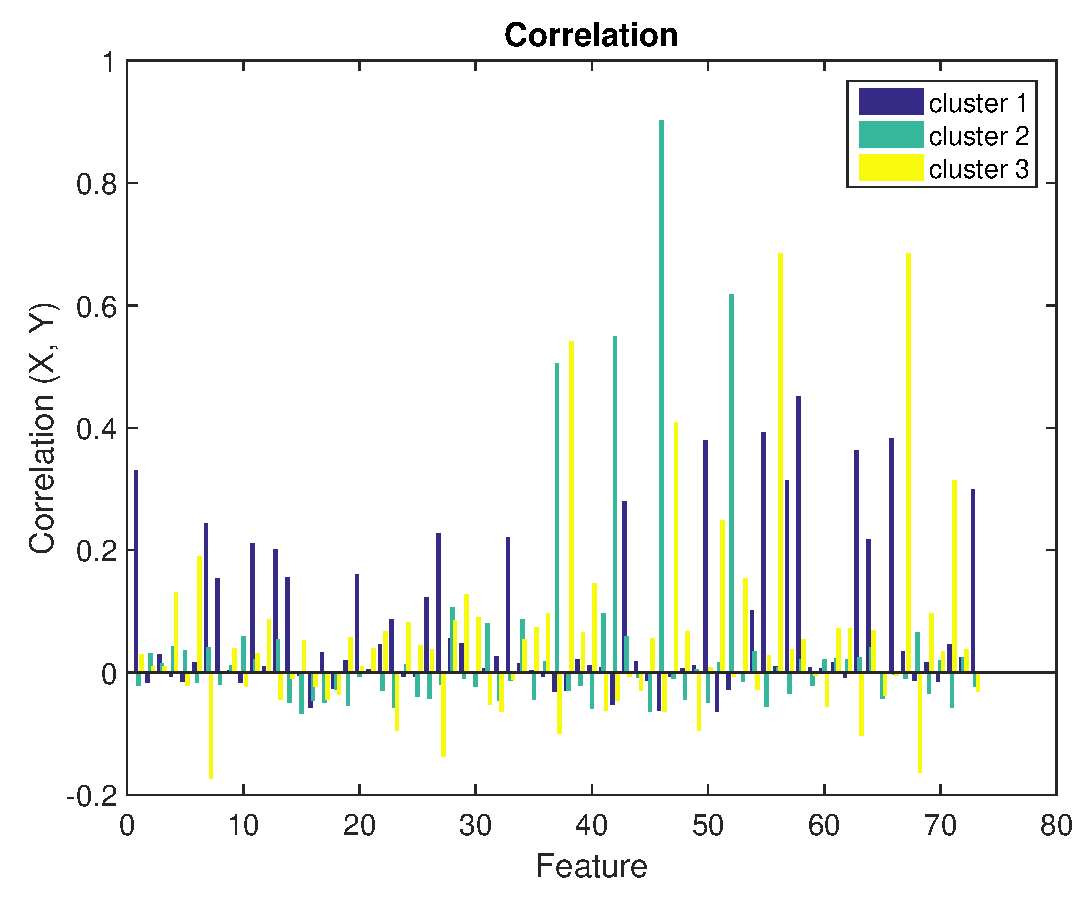
\includegraphics[width=2.5in]{figures/corr_cropped.pdf} \label{fig:corr}}
\subfigure[Feature with higher correlation in the cluster 2]{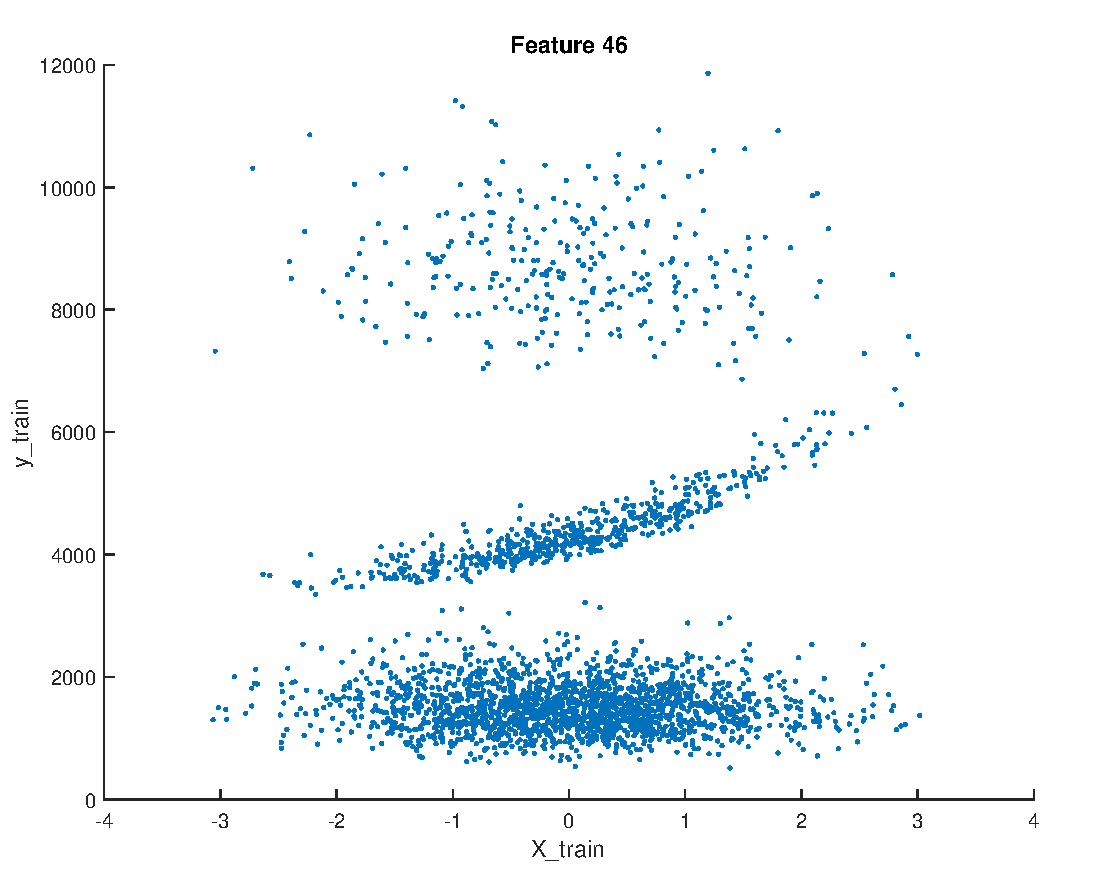
\includegraphics[width=2.5in]{figures/ft46.pdf} \label{fig:ft46}}
\caption{Correlations between Input and Output data}
\end{figure}

We also used dummy encoding for all categorical variables in both regression and classification datasets.


\section{Regression}

\subsection{Logistic Regression}
First we classified the data into three clusters. We used two relevant features shown in figure \ref{fig:rlvtft} to separate the inputs in the first and the third clusters respectively. Once we have determined which inputs of the training set belong to which cluster, we applied logistic regression in the three clusters. The average errors for each regression are shown in the table \ref{table:errTable}.

\begin{figure}[!h]
\center
\subfigure{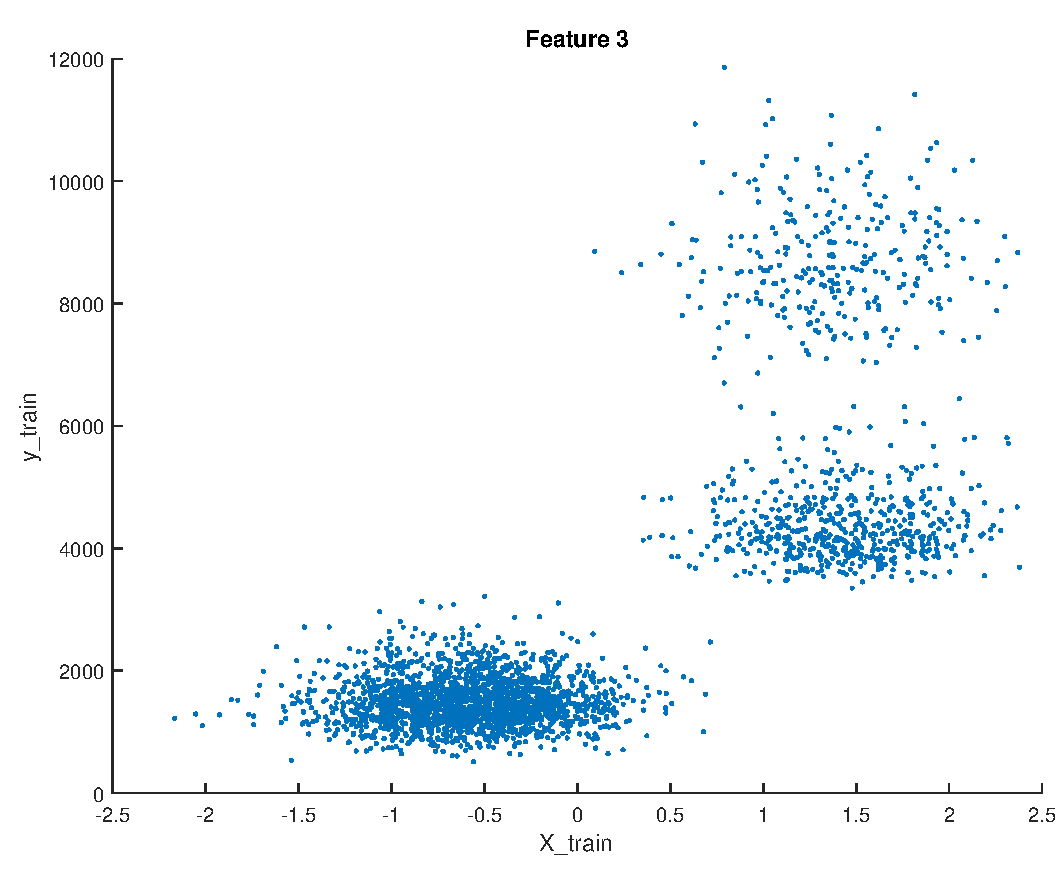
\includegraphics[width=2.5in]{figures/ft3.pdf} \label{fig:ft3}}
\subfigure{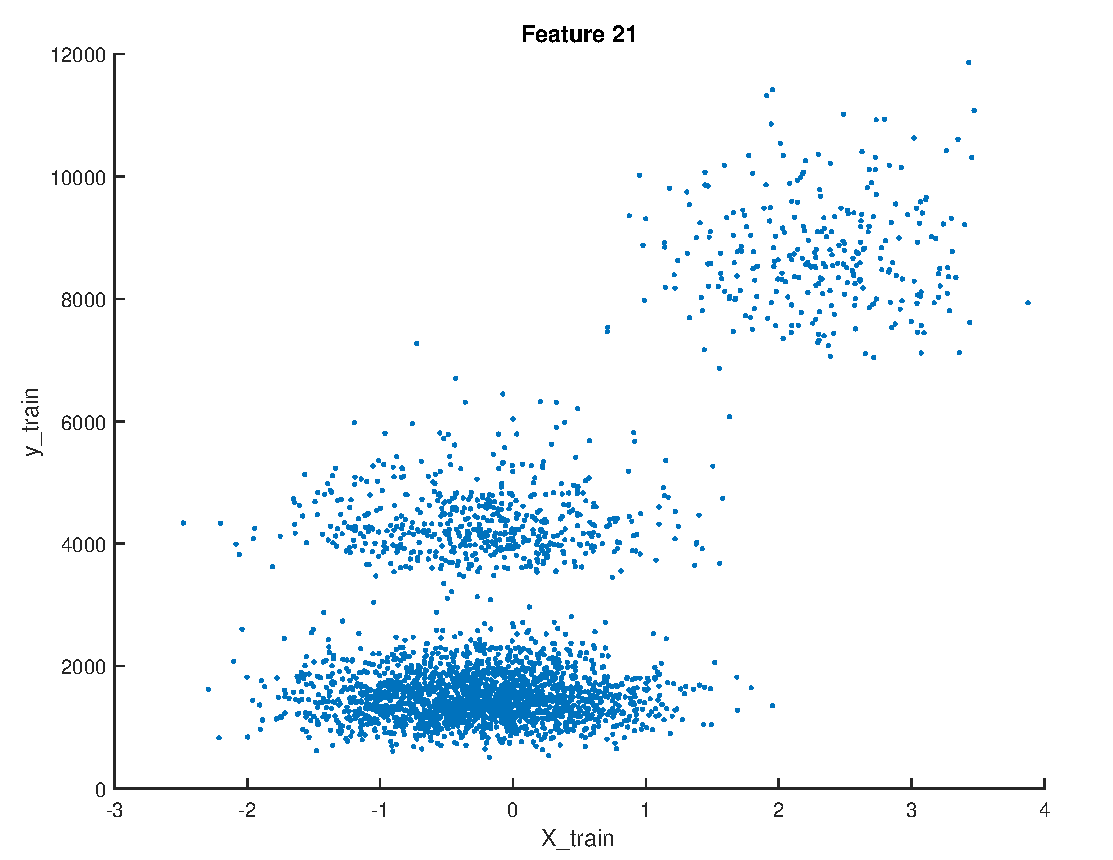
\includegraphics[width=2.5in]{figures/ft21.pdf} \label{fig:ft21}}
\caption{Scatter Plots of Regression Output $\mathbf{y\_train}$}
\label{fig:rlvtft}
\end{figure}

\begin{table}[!h]
\begin{center}
\begin{tabular}{|c||c|c|c|}
    \hline
    Clusters & Training error & Test error  \\
    \hline\hline
    Cluster 1 &$12.650$ & $12.624$ \\
    \hline
    Cluster 2 &$12.565$&$12.567$ \\
    \hline
    Cluster 3 &$10.614$&$10.554$ \\
    \hline
\end{tabular}
\caption{RMSE with Logistic Regression}
\label{table:errTable}
\end{center}
\end{table}


For each testing point, we computed the probability that it belongs to a cluster with the betas obtained from logistic regression. We therefore classified each point in the cluster with the higher probability.

\subsection{Ridge Regression and Feature Transformation}
The next step was to apply a different model of regression depending on the cluster to which the input belongs to. For all three models, we chose ridge regression but we tried different models (with all features or with a subset of features and with or without feature transformation). All categorical variables were dummy encoded.

For the first cluster, we found that ridge regression with all features and without feature transformation gave the best result.
We thought that choosing features with a high correlation would fit better to the model but the difference wasn't significant.
For the second cluster, we found that ridge regression with all features gave the best result. We improved the performance by taking the square of the $46^{th}$ feature $(X_{46})^{2}$. 

For the third cluster, we found that ridge regression with all features gave the best result. We improved the performance by taking the square of the $38^{th}$ feature $(X_{38})^{2}$ and of the $56^{th}$ feature $(X_{56})^{2}$. 

Figure \ref{fig:lambda} shows that we optimized the error with lambda equals to 15.
The table \ref{table:errTableClst} shows the average error for training and test set of the best model fitting each cluster with $lambda = 2$

\begin{figure}[!h]
\center
\subfigure[Correlation]{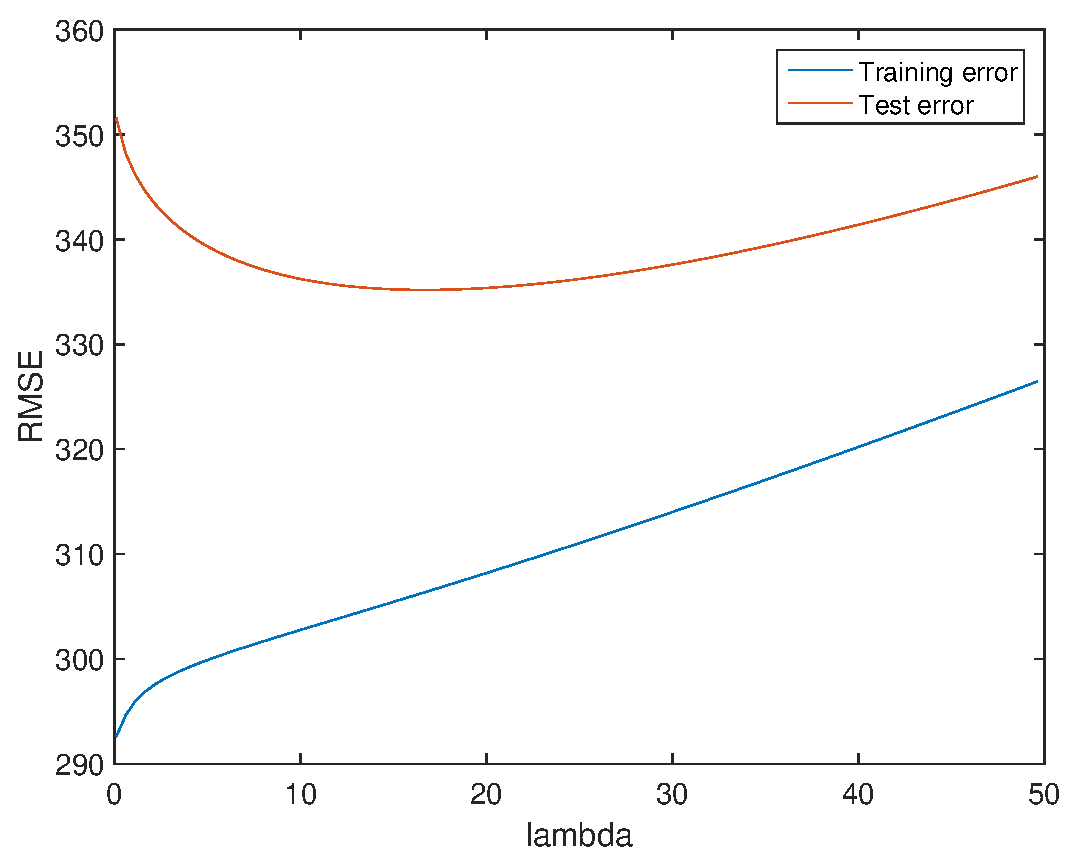
\includegraphics[width=2.5in]{figures/cl3lambda_cropped.pdf} \label{fig:lambda}}
\caption{}
\end{figure}

\begin{table}[!h]
\begin{center}
\begin{tabular}{|c||c|c|c|}
    \hline
    Best Model of cluster & Training error & Test error  \\
    \hline\hline
    Model of cluster 1 &$144.294$ & $151.978$ \\
    \hline
    Model of cluster 2 &$72.059$&$82.874$ \\
    \hline
    Model of cluster 3 &$127.720$&$184.616$ \\
    \hline
\end{tabular}
\caption{Average RMSE of models}
\label{table:errTableClst}
\end{center}
\end{table}


\section{Classification}

\subsection{Logistic Regression}

In classifying our data, we think that the application of logistic regression is well-suited in this specific setting. The dimensionality of input matrix $D= 28$ doesn't exceed the number of data points $N = 1500$ $\mathbf{D\ll N}$. Therefore, we are not in the case where infinitely many solutions exists because the number of unknowns are smaller than the number of equations. We don't need to regularize our problem since there is low variance as shows figure \ref{fig:ClassPlot}.

We tried logistic regression with different parameters to find the best model to fit classification data and make predictions with minimal rmse, log loss and 0-1 loss errors. As in regression, we normalized non-categorical variables and dummy encoded categorical variables. We used cross validation with different values of K and tried different values of alpha to plot learning curve corresponding to the train and test errors versus alpha. We got the best value for 0-1 error (approximately $8.480000e^{-02}$) when using logistic regression with alpha value: $4.005000e^{-03}$ and with no feature transformation. 

\begin{figure}[!h]
\center
\subfigure[Scatter Plot of Classification Data]{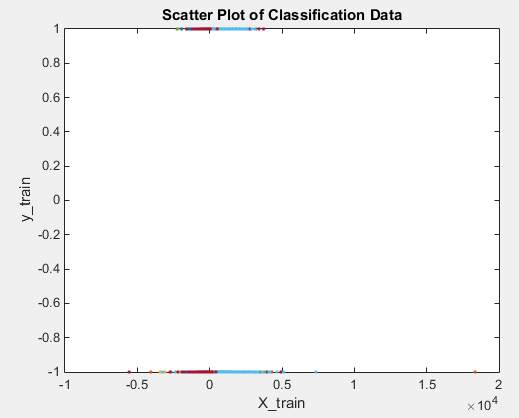
\includegraphics[width=2.5in]{figures/ClassificationPlot.PNG} \label{fig:ClassPlot}}
\subfigure[Logistic Regression using 4-fold Cross Validation]{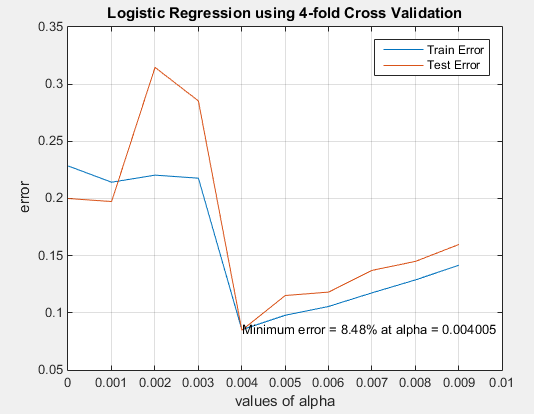
\includegraphics[width=2.5in]{figures/crossValidationClass.PNG} \label{fig:crossValid}}
\caption{Classification of data using logistic regression}
\end{figure}

\subsection{Feature Transformation}
We tried using different methods of feature transformation, like taking all the elements of the input matrix $\mathbf{X\_train}$ to power of 1/2, 2, 3 etc or using log. However, we didn't observe any significant improvement. So, we used only normalization and dummy encoding. 

\section{Summary}
In this project, we analyzed regression and classification data set. We used cross-validation with K-Fold to test our models and compute the average error for the training set and the test set.

We tried different methods to find the best model minimizing the error and fitting at best with our data. We thought that selecting a relevant subset of features in our data which appear to be higher correlated with the output values minimizes the error. But we saw that the difference of the errors isn't significant. Finally, our best model with ridge regression has a average RMSE of 714.09.

We used logistic regression to classify our data and got the best value for 0-1 error (approximately $8.480000e^{-02}$) when using alpha value: $4.005000e^{-03}$. The use of feature transformation didn't make any significant improvement. 


\subsubsection*{Acknowledgments}
We would like to thank Dr. Mohammed Emtiyaz Khan for giving us the opportunity to work on this project which provided us with a rich learning experience and a great insight of what machine learning entails in the practical world. We also appreciate the help of all TAs and people we talked to during the labs. Without their help, our project could not have be done this way and we couldn't have figured out the correct transitions from theory to code. We collaborated as a team by writing the functions, trying the methods and writing the report together to be able to discuss the results.   

\subsubsection*{References}

Advice for Applying Machine Learning http://cs229.stanford.edu/materials/ML-advice.pdf

Feature Engineering: http://machinelearningmastery.com/discover-feature-engineering-how-to-engineer-features-and-how-to-get-good-at-it/

A Few Useful Things to Know about Machine Learning: http://homes.cs.washington.edu/~pedrod/papers/cacm12.pdf

http://www.maths.tcd.ie/~dwilkins/LaTeXPrimer/ - tutorial on Latex

http://www.stdout.org/~winston/latex/latexsheet-a4.pdf - cheat sheet with useful commands for Latex

http://mirror.switch.ch/ftp/mirror/tex/info/first-latex-doc/first-latex-doc.pdf - example how to create a document with Latex

http://en.wikibooks.org/wiki/LaTeX - detailed tutorial on Latex



\end{document}
